\section{Mathematical model}\label{sec:Math_model}

\subsection{Porous medium deformation and fracture propagation}\label{Sec:Phase_Field}
In this section, 
we briefly recapitulate the basic notations and the underlying equations of the phase field method for pressurized fractures in brittle materials.

\subsubsection{Variational formulation of brittle fracture}
Let $\Omega\subset\mathbb{R}^\eta$, $\eta=2,3$ be an open Lipchitz domain occupied by a porous medium with a lower-dimensional fracture $\mathcal{C}\in\mathbb{R}^{\eta-1}$, see Figure \ref{Fig:comput_domain}. Let the displacement field be $\bm{u}:\Omega\rightarrow\mathbb{R}^\eta$. Let $\Gamma_D,\Gamma_N\subseteq \partial\Omega$ be such that $\Gamma_D\cup\Gamma_N=\partial\Omega$ and $\Gamma_D\cap\Gamma_N=\emptyset$. Further, let $\bm{u}_D: \Gamma_D\rightarrow\mathbb{R}^2$ and $\bm{t}_N: \Gamma_N\rightarrow\mathbb{R}^2$ be prescribed displacement and traction boundary conditions, respectively. We denote by $\Gamma_B$ the boundary of a borehole, and by $Q_g:\Gamma_B\rightarrow\mathbb{R}$ the fluid source. We have $\Gamma_P=\partial\Omega\setminus\Gamma_B$, and let $p_D:\Gamma_p\rightarrow\mathbb{R}$ be prescribed pressure. Also, $\mathbf{b}:\Omega\rightarrow\mathbb{R}^\eta$ is the body force per unit volume exerted to the solid.
\begin{figure}[htbp]
	\centering
	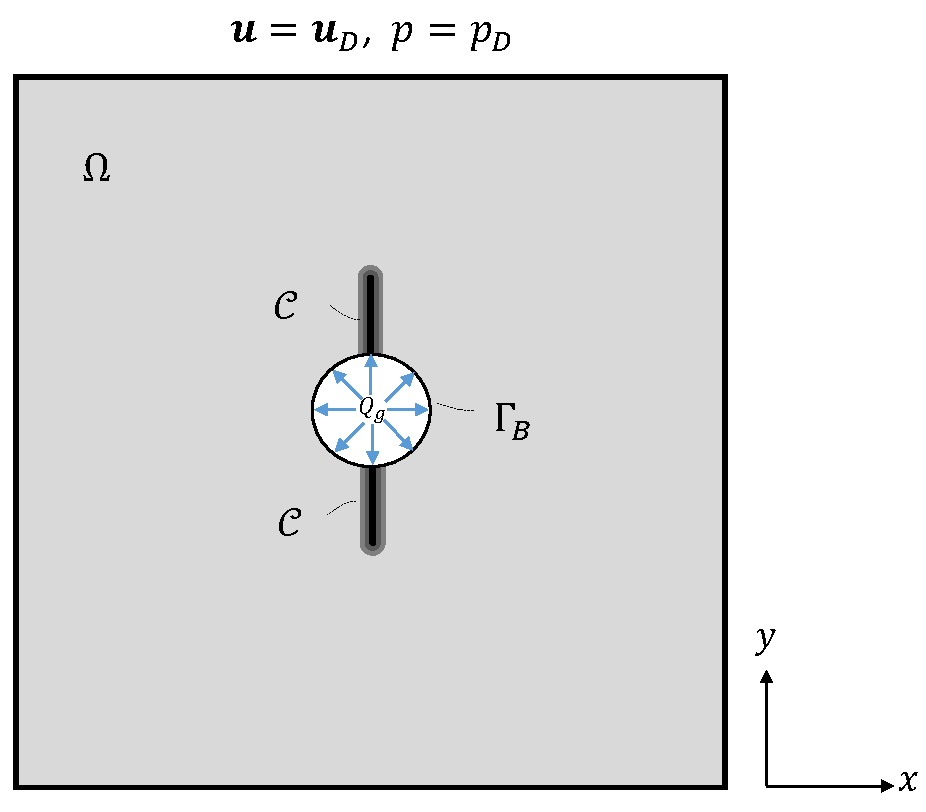
\includegraphics[width=0.8\textwidth]{omega_insitu2}
	\caption{A bounded reservoir domain $\Omega$ with a lower-dimensional crack $\mathcal{C}\in\mathbb{R}^{\eta-1}$ (left) and its diffuse approximation.}
	\label{Fig:comput_domain}
\end{figure}
\comment{We also need to define prescribed boundary condition for $T$.}
The linearized strain tensor takes the form:
\begin{equation}\label{Eq:epsilon}
	\begin{aligned}
		\bm{\varepsilon}(\bm{u})=\frac12(\nabla\bm{u}+\nabla\bm{u}^T)
	\end{aligned}
\end{equation}
which can be decomposed into two parts:
\begin{equation}\label{Eq:epsilon_decomp}
\begin{aligned}
	\bm{\varepsilon}(\bm{u}) = \bm{\varepsilon_e}+\bm{\varepsilon_{\theta}}.
\end{aligned}
\end{equation}
Here, $\bm{\varepsilon_e}$ and $\bm{\varepsilon_{\theta}}$ are the elastic and thermal strain tensors, respectively. We assume that $\bm{\varepsilon_{\theta}}$ is proportional to the temperature $\theta$ via:
\begin{equation}\label{Eq:epsilon_theta}
	\begin{aligned}
		\bm{\varepsilon_{\theta}} = \beta(\theta-\theta_0)\mathbf{I},
	\end{aligned}
	\end{equation}
where $\theta_0$ is a reference temperature, $\beta$ is the linear expansion coefficient of the material, and $\mathbf{I}$ is the \deleted{second-order} identity tensor.

The energy of a poroelastic medium $\Omega$ with a crack $\mathcal{C}$ reads:
\begin{equation}\label{Eq:E}
\begin{aligned}
E(\bm{u},\mathcal{C}):= \frac12 \int_{\Omega\setminus\mathcal{C}} \mathbb{C}\left(\bm{\varepsilon}_e(\bm{u})-\frac{\alpha}{3K}p\mathbf{I}\right):\left(\bm{\varepsilon}_e(\bm{u})-\frac{\alpha}{3K}p\mathbf{I}\right)\; d\Omega - W(\bm{u}),
\end{aligned}
\end{equation}
where $\mathbb{C}\in\mathbb{R}^4$ denotes the fourth-order Gassman tensor, and $\alpha\in[0,1]$ and $p$ are the Biot's coefficient and the pore pressure, respectively. Also, $K=E/[3(1-2\nu)]$ where $E$, $\nu$ are Young's modulus and Poisson's ratio, respectively.
The external work $W(\bm{u})$ is defined as:
\begin{equation}\label{Eq:External}
	\begin{aligned}
		W(\bm{u}):=\int_{\Omega} \bm{b} \cdot \bm{u} \; d\Omega+\int_{\Gamma_N} \bm{t}_N\cdot \bm{u} \; d\Gamma - \int_{\mathcal{C}} p\bm{n}\cdot[\bm{u}] \; d\Gamma,
	\end{aligned}
\end{equation}
where $\bm{n}\cdot[\bm{u}]\geq 0$ represents the displacement discontinuity on the fracture surface so that the term $\int_{\mathcal{C}} p\bm{n}\cdot[\bm{u}] \; d\Gamma$
%third term on the right hand side of \eqref{Eq:External}
is the work done by the absorbed gas on the fracture surface.

The variational approach to fracture first proposed by Francfort and Marigo \cite{bourdin2008variational} defines the total energy as the sum of the potential energy and the surface energy required to create a fracture set $\mathcal{C}$. Let $\mathcal{H}^{\eta-1}(\mathcal{C})$ denote the lower-dimensional Hausdorff measure of $\mathcal{C}$. Taking the constant $G_c\in\mathbb{R}^+$ as the strain energy released per unit length of fracture extension, the total energy will be formed as:
\begin{equation}\label{Eq:Pi}
	\begin{aligned}
		\Pi[\bm{u},\mathcal{C}]=E(\bm{u},\mathcal{C})+G_c\mathcal{H}^{\eta-1}(\mathcal{C}).
	\end{aligned}
\end{equation}
In the variational setting, the Griffith criteria will be the
minimum of the total energy \eqref{Eq:Pi} with respect to any admissible displacement field $\bm{u}$ and any fracture set $\mathcal{C}$ subject to an irreversibility condition, i.e., the crack can never heal.

\subsubsection{Regularized variational formulation of brittle fracture}
To develop a numerical method to approximate \eqref{Eq:Pi}, we need to replace the sharp description of crack $\mathcal{C}$ with a phase field representative, where the phase field is denoted as $d:\Omega\rightarrow[0,1]$. Following the approach presented by Ambrosio and Tortorelli \cite{ambrosio1990approximation, ambrosio1992approximation}, one can approximate $\mathcal{H}^{\eta-1}(\mathcal{C})$ with the help of an elliptic functional as:
\begin{equation}\label{Eq:Gamma_ell}
\begin{aligned}
\mathcal{C}_\ell[d]:=\frac{1}{4c_{\omega}}\int_\Omega\left(\frac{\omega(d)}{\ell} + \ell \nabla d\cdot\nabla d\right) d\Omega,  
\end{aligned}
\end{equation}
%where $d:\Omega\rightarrow[0,1]$ is the phase field parameter. 
In particular, regions with $d = 0$ and $d = 1$ correspond to the intact and fully broken materials, respectively.
We denote by $\ell>0$ the regularization length scale, which may also be interpreted as a material property, e.g., the size of the process zone.
In \eqref{Eq:Gamma_ell}, we consider $c_\omega=\int_{0}^{1} \sqrt{\omega(d)}$ as a normalization constant such that as $\ell\rightarrow 0$, $\mathcal{C}_\ell[d]$ converges to the length of sharp crack $\mathcal{H}^{\eta-1}(\mathcal{C})$. Also, we choose $\omega(d)=d^2$, see \cite{tanne2018crack, Bourdin2014014301} for more elaborations.

The solid endures partial loss of stiffness due to the presence of fractures. To model this effect, the poroelastic energy needs to be degraded with respect to the evolution of the phase field. Also note that as the damaged material responds differently to tension and compression, we should let only a part of the poroelastic energy be degraded. Following \cite{amor2009regularized}, we assume that both volumetric expansion and deviatoric deformation contribute to crack propagation but not volumetric compression. 
A decomposition of $\bm{\varepsilon}_e$ into volumetric and deviatoric components reads:
\begin{equation}
	\begin{aligned}
		\vol\bm{\varepsilon}_e := \frac{1}{\eta} (\trace\bm{\varepsilon}_e) \mathbf{I}_{\eta}, \quad
		\dev\bm{\varepsilon}_e := \bm{\varepsilon}_e - \vol\bm{\varepsilon}_e,
	\end{aligned}
\end{equation}
where $\vol\bm{\varepsilon}_e$ will also be decomposed into expansion and compression parts such that
\begin{equation}
	\begin{aligned}
		\vol\bm{\varepsilon}_e=\vol_+\bm{\varepsilon}_e+\vol_-\bm{\varepsilon}_e, \quad \vol_{\pm}\bm{\varepsilon}_e=\frac{1}{\eta}\langle \trace \bm{\varepsilon}_e \rangle_{\pm},
	\end{aligned}
\end{equation}
where $\langle a\rangle_\pm:=\left(|a|\pm a\right)/2$ for all $a\in\mathbb{R}$.
%On this basis, we can rewrite \eqref{Eq:E} as:
On this basis, we rewrite \eqref{Eq:E} with decomposition of the poroelastic energy into expansion/compression volumetric and deviatoric parts as:
\begin{equation*}\label{Eq:E_Amor}
	\begin{aligned}
		E(\bm{u},\mathcal{C})&:= \frac12 \int_{\Omega\setminus\mathcal{C}} \mathbb{C}\Big\langle\vol\bm{\varepsilon}_e-\frac{\alpha}{3K}p\mathbf{I}\Big\rangle_{+}:\Big\langle\vol\bm{\varepsilon}_e-\frac{\alpha}{3K}p\mathbf{I}\Big\rangle_{+}\; d\Omega \\&+
		\frac12 \int_{\Omega\setminus\mathcal{C}} \mathbb{C}\Big\langle\vol\bm{\varepsilon}_e-\frac{\alpha}{3K}p\mathbf{I}\Big\rangle_{-}:\Big\langle\vol\bm{\varepsilon}_e-\frac{\alpha}{3K}p\mathbf{I}\Big\rangle_{-}\; d\Omega \\&+ \int_{\Omega\setminus\mathcal{C}} \mathbb{C}\dev\bm{\varepsilon}_e:\dev\bm{\varepsilon}_e\; d\Omega - W(\bm{u}),
	\end{aligned}
\end{equation*}
To take into account any pre-existing crack, we define $\Gamma_d\subset\overline{\Omega}$ to be a set with Hausdorff dimension $\eta-1$, and $d_0:\Gamma_d\rightarrow[0,1]$ as the Dirichlet boundary condition for $d$. Thus, we define the affine space of the admissible $\bm{u}$ and $d$ fields:
\begin{equation}\label{Eq:Dissipative_admissible}
\begin{aligned}
\mathscr{S}_u &:= \left\{\bm{u}\in H^1\left(\Omega; \mathbb{R}^\eta\right) \middle|
\bm{u} = \bm{u}_D \text{ on } \Gamma_D
\right\}, \\
\mathscr{S}_d &:= \left\{d\in H^1(\Omega) \middle|
0 \le d \le 1 \text{ a.e.}, d = d_0 \text{ on } \Gamma_d
\right\}. \\
%\mathscr{S}_d &:= H^1(\Omega).
\end{aligned}
\end{equation}
On this basis, the regularized variational formulation for brittle fracture of the solid reads: Find $\left(\bm{u}\times d \right)\in\mathscr{S}_{\bm{u}}\times\mathscr{S}_d$ that minimizes the following total energy:
\begin{equation}\label{Eq:Dissipative_functional}
\begin{aligned}
\Pi(\bm{u},d)&:= \frac12 \int_{\Omega} \mathbb{C}\Big\langle\sqrt{g(d)}\vol\bm{\varepsilon}_e-\frac{\alpha}{3K}p\mathbf{I}\Big\rangle_{+}:\Big\langle\sqrt{g(d)}\vol\bm{\varepsilon}_e-\frac{\alpha}{3K}p\mathbf{I}\Big\rangle_{+}\; d\Omega \\&+
\frac12\int_{\Omega}\mathbb{C}\Big\langle\vol\bm{\varepsilon}_e-\frac{\alpha}{3K}p\mathbf{I}\Big\rangle_{-}:\Big\langle\vol\bm{\varepsilon}_e-\frac{\alpha}{3K}p\mathbf{I}\Big\rangle_{-}\; d\Omega \\&+
\int_{\Omega} g(d)\mathbb{C}\dev\bm{\varepsilon}_e:\dev\bm{\varepsilon}_e\; d\Omega\\&+
\frac{G_c}{4c_{\omega}}\int_\Omega \left(\frac{\omega(d)}{\ell} + \ell \nabla d\cdot\nabla d\right)\;d\Omega- W(\bm{u}),
\end{aligned}
\end{equation}
where $g(d)$ is a degradation function that satisfies $g(0)=1$, $g(1)=0$, and $g'(d)<0$. A usual choice is $g(d)=(1-d)^2$ \cite{Bourdin2000797}. Note that the requirement $g'(d)<0$ comes from the underlying irreversibility condition (the fracture can never heal) in time:
\begin{equation}\label{Eq:irreversibility}
\partial_t d\geq 0.
\end{equation}
Consequently, modeling of fracture evolution problems leads to {inequality constraints, and sometimes gives rise to a variational inequality formulation}.
Also, note that in this regularized form, the external work in \eqref{Eq:External} is rewritten as:
\begin{equation*}
\begin{aligned}
W(\bm{u}):=\int_{\Omega} \bm{b} \cdot \bm{u} \; d\Omega+\int_{\Gamma_N} \bm{t}_N\cdot \bm{u} \; d\Gamma - \int_{\Omega} p\bm{u}\cdot\nabla d \; d\Omega,
\end{aligned}
\end{equation*}
where $\int_{\Omega} \bm{u}\cdot\nabla d \; d\Omega$ represents the fracture volume \cite{BourdinCFRAC13}.

It can be shown that when $\ell\rightarrow 0$, the regularized formulation $\Gamma-$converges to that with explicit crack representation, i.e., when $\ell\rightarrow0$, the solution to the minimization problem \eqref{Eq:Dissipative_functional} $\Gamma$-converges to that of $d\Pi[\bm{u},\mathcal{C}]=0$, and also $\mathcal{C}_\ell[d]$ converges to $\mathcal{H}^{\eta-1}(\mathcal{C})$. See Bourdin \emph{et al.} \cite{bourdin2008variational} for the proof of the static anti-plane case.

%\paragraph{The choice of $\ell$}
%{Based on an analytical solution for the critical tensile strength $\sigma_\text{cr}$ that a one-dimensional bar can sustain \cite{Bourdin2014014301}, we use the following equation for the choice of $\ell$:}
%\begin{equation}\label{Eq:choice_ell}
%    \begin{aligned}
%        \ell=\frac{3EG_c}{8\sigma_\text{cr}^2},
%    \end{aligned}
%\end{equation}
%where $E$ and $g_c$ can be obtained from regular experiments, while $\sigma_\text{cr}$ can be approximated by the tensile strength $\sigma_t$. Assuming all {other} parameters are known, the formula \eqref{Eq:choice_ell} is able to estimate $\ell$, though the accuracy is unknown for more complex cases.

\subsection{Carbon dioxide as a compressible fluid} \label{Sec:CO2}
Assume the porous medium is saturated by a single-phase gas. We denote by $\phi$ the porosity of the porous medium (the fraction of volume occupied by the gas), and by $\rho_g, \rho_s$ the gas and solid density, respectively. Note that in this paper, the subscripts $s$  and $g$ refer to solid and gas phases, respectively. The mass balance for the gas reads:
\begin{equation}\label{Eq:Mass_fluid}
    \begin{aligned}
        \partial_t\left(\phi\rho_g\right)  +\nabla\cdot\left(\phi\rho_g \mathbf{v}_g\right)&=0  \quad  &\text{in~} \Omega,
    \end{aligned}
\end{equation}
and for the solid phase:
\begin{equation}\label{Eq:Mass_solid}
\begin{aligned}
\partial_t\left(\left(1- \phi\right) \rho_s\right) + \nabla\cdot\left(\left(1- \phi\right)\rho_s \mathbf{v}_s\right)&=0  \quad  &\text{in~} \Omega.
\end{aligned}
\end{equation}
In \eqref{Eq:Mass_fluid} and \eqref{Eq:Mass_solid}, $\mathbf{v}_g$ and $\mathbf{v}_s$ are respectively the absolute value of gas and solid velocity in the bulk.
Multiplying \eqref{Eq:Mass_fluid} by $\frac{1}{\rho_g}$ and \eqref{Eq:Mass_solid} by $\frac{1}{\rho_s}$, we sum up \eqref{Eq:Mass_fluid} and \eqref{Eq:Mass_solid} to obtain:
\begin{equation*}\label{Eq:Mass_sum}
	\begin{aligned}
	&\frac{\phi}{\rho_g}\partial_t\rho_g+\frac{1}{\rho_g}\nabla\cdot\left(\phi\rho_g \mathbf{v}_g\right)+\frac{1-\phi}{\rho_s}\partial_t\rho_s\\
	&+\frac{1}{\rho_s}\left[(1-\phi)\rho_s \nabla \cdot \mathbf{v}_s+\mathbf{v}_s \cdot \nabla \left((1-\phi)\rho_s)\right)\right]=0.
	\end{aligned}
\end{equation*}
By neglecting $\nabla\left(\left(1-\phi\right)\rho_s\right)$, it reads:%(see \cite{lewis1998finite}, section 2.6.3.2),
\begin{equation}\label{Eq:Mass_sum_intmediate}
	\begin{aligned}
        \frac{\phi}{\rho_g }\partial_t\rho_g+\frac{1}{\rho_g}\nabla\cdot\left(\phi\rho_g \mathbf{v}_g\right)+\frac{1-\phi}{\rho_s}\partial_t\rho_s+(1-\phi)\nabla\cdot \mathbf{v}_s=0.
	\end{aligned}
\end{equation}
We introduce an intermediate term $\nabla\cdot\left(\phi\rho_g\mathbf{v}_s\right)$ as follows:
\begin{equation*}
	\begin{aligned}
    	\frac{1}{\rho_g}\nabla\cdot\left(\phi\rho_g \mathbf{v}_s\right)=\frac{1}{\rho_g}\left[\phi\rho_g\nabla\cdot\mathbf{v}_s+\mathbf{v}_s \cdot \nabla\left(\phi\rho_g\right)\right] \approx \phi\nabla\cdot\mathbf{v}_s,
    \end{aligned}
\end{equation*}
Having this, we define $\nabla\cdot\left(\phi\rho_g\mathbf{v}_g\right)$ as:
\begin{equation} \label{Eq:div_vrho_f}
	\begin{aligned}
	    \frac{1}{\rho_g}\nabla\cdot\left(\phi\rho_g\mathbf{v}_g\right)
    	&=\frac{1}{\rho_g}\nabla\cdot\left(\phi\rho_g \mathbf{v}_g\right)-\frac{1}{\rho_g}\nabla\cdot\left(\phi\rho_g \mathbf{v}_s\right)+\phi\nabla\cdot\mathbf{v}_s\\
	    &=\frac{1}{\rho_g}\nabla\cdot\left[\phi\rho_g\left(\mathbf{v}_g-\mathbf{v}_s\right)\right]+\phi\nabla\cdot\mathbf{v}_s.
    \end{aligned}
\end{equation}
By substituting \eqref{Eq:div_vrho_f} in \eqref{Eq:Mass_sum_intmediate}, we obtain:
\begin{equation}\label{Eq:Mass_Conserv_sum_darcy}
\begin{aligned}
\frac{\phi}{\rho_g}\partial_t\rho_g +\frac{1-\phi}{\rho_s}\partial_t\rho_s+\nabla\cdot\mathbf{v}_s+\frac{1}{\rho_g} \nabla\cdot \left[\phi \rho_g \left(\mathbf{v}_g-\mathbf{v}_s \right)\right] =0,  \quad  &\text{in~} \Omega.
\end{aligned}
\end{equation}
%We will rewrite each term of \eqref{Eq:Mass_Conserv_sum_darcy} in terms of $\bm{u}, p, T$.
The first term on the left hand side of \eqref{Eq:Mass_Conserv_sum_darcy} can be written as:
\begin{equation}\label{Eq:diff_rho_f}
\begin{aligned}
\frac{\phi}{\rho_g}\partial_t\rho_g = \frac{\phi}{\rho_g} \left[ \frac{\partial \rho_g}{\partial p}\partial_t p+\frac{\partial \rho_g}{\partial T}\partial_tT\right] = \phi \left[ \beta_p \partial_t p+ \beta_T \partial_tT\right],
\end{aligned}
\end{equation}
where $\beta_p=\rho_g{\partial\rho_g}/{\partial p}$, and $\beta_T=\rho_g{\partial\rho_g}/{\partial T}$.
%\comment{Here, I should see if there is a name for $\beta_p$, $\beta_T$.}
Under non-isothermal conditions, the gas density varies significantly with both pressure and temperature. We {capture} this by an equation of state (EOS) \cite{mahmoud2014development}:
\begin{equation} \label{Eq:EOS}
\rho_g\left( p,T\right)  =\frac{Mp}{Z\left( p,T\right) RT},
\end{equation}
where $M$ denotes the gas molecular weight, and $R$ is the general gas constant. Also, $Z$ is obtained from the following:
\begin{equation*} \label{Eq:Z_EOS}
Z=\left(0.702e^{-2.5T_{pr}} \right) p_{pr}^2 -\left(5.52e^{-2.5T_{pr}} \right) p_{pr}+\left(0.044 T_{pr}^2 -0.164T_{pr} +1.15\right).
\end{equation*}
Here, $p_{pr}=p/p_c$ and $T_{pr}=T/T_c$ are the reduced pressure and temperature, respectively. Note also $p_c$ and $T_c$ denote the critical pressure and temperature.
On this basis, we rewrite $\beta_p$ and $\beta_T$ as follows:
\begin{equation} \label{Eq:partial_density_p_T}
\begin{aligned}
\beta_p=\frac{1}{\rho_g}\frac{\partial \rho_g}{\partial p} &= \frac{1}{p}- \frac{1}{Z} \frac{\partial Z}{\partial p}, \\
\beta_T= \frac{1}{\rho_g}\frac{\partial \rho_g}{\partial T} &= -\frac{1}{T}- \frac{1}{Z} \frac{\partial Z}{\partial T}.
\end{aligned}
\end{equation}
The second term on the left hand side of \eqref{Eq:Mass_Conserv_sum_darcy} reads \cite{lewis1998finite}: %see \cite{lewis1998finite}, Equation 2.190)
\begin{equation}\label{Eq:diff_rho_s}
\begin{aligned}
\frac{1-\phi}{\rho_s} \partial_t\rho_s= \left(\alpha-\phi \right) \frac{1}{K_s} \partial_t p -\beta_s\left(\alpha-\phi \right) \partial_t T - \left(1-\alpha \right)  \nabla \cdot \mathbf{v}_s,
\end{aligned}
\end{equation}
%\comment{Is $K_s$ the same as $k$ in \eqref{Eq:E}?}
where {$K_s$ denotes the bulk modulus of the grain material}, $\beta_s=\frac{1}{\rho_s}\frac{\partial\rho_s}{\partial T}$ is the thermal expansion coefficient for the solid, and $T$ is the absolute temperature.
The third term on the left hand side of \eqref{Eq:Mass_Conserv_sum_darcy} (also the last term of \eqref{Eq:diff_rho_s}) can be written as follows \cite{merxhani2016introduction}:
\begin{equation} \label{Eq:solid velocity}
\begin{aligned}
\nabla \cdot \mathbf{v}_s=\nabla \cdot \dot{\bm{u}}= \dot{\left( \nabla \cdot \bm{u}\right)}=\partial_t\left(\vol\bm{\varepsilon}\right).
\end{aligned}
\end{equation}
The forth term on the left hand side of \eqref{Eq:Mass_Conserv_sum_darcy} can be written in the form of Darcy's law. This law indicates a linear relationship between the relative velocity of gas to solid and the head pressure gradient:
\begin{equation}\label{Eq:Darcy_law}
\begin{aligned}
\mathbf{q} = \phi \left(\mathbf{v}_g-\mathbf{v}_s \right) = -\frac{\kappa}{\mu} \nabla p,
\end{aligned}
\end{equation}
where $\kappa$ is the permeability of rock, and $\mu$ is the dynamic fluid viscosity. 
Note that we neglect the effect of gravity in Darcy's law. %($\rho_f g \nabla z$)

By substituting \eqref{Eq:diff_rho_f}, \eqref{Eq:diff_rho_s}, \eqref{Eq:solid velocity}, and \eqref{Eq:Darcy_law} in \eqref{Eq:Mass_Conserv_sum_darcy}, the governing equation for CO$_2$ flow is written as follows:
\begin{equation}\label{Eq:General_pressure}
\begin{aligned}
\left[\phi\beta_p +\frac{\alpha-\phi}{K_s}\right]\partial_t p+\left[\phi\beta_T-\beta_s(\alpha-\phi)\right]\partial_t T\\+\alpha \partial_t(\vol\varepsilon)+\frac{1}{\rho_g}\nabla\cdot \left(\rho_g\mathbf{q}\right)=0 \quad &\text{in~} \Omega,\\
\rho_g\bm{q} \cdot \mathbf{n} =-Q_g \quad  &\text{on~} \Gamma_B,\\
p = p_D \quad &\text{on~}\Gamma_P.
\end{aligned}
\end{equation}
%where $\Gamma_P=\partial\Omega\setminus\Gamma_B$.
\subsubsection{Calculation of $k$}
\paragraph{Change of $k$ by phase field} As the cracks initiates, the permeability of the solid matrix increases inside the crack. To incorporate this effect into our model, 
we correlate the permeability to phase field by:
\begin{equation} \label{Eq:k_0}
\kappa(d)=\kappa_0+d\left(\kappa_c-\kappa_0 \right),
\end{equation}
where $\kappa_0$, $\kappa_c$ are the permeability of the intact material and the crack, respectively. Hence, a change of permeability is assumed between the intact porous medium ($d=0$) and the crack ($d=1$). In \eqref{Eq:k_0}, $\kappa_c={w_c^2}/{12}$ where $w_c$ is the fracture width.
Let $h_e$ be the mesh size, $\varepsilon_{ii}$ be the components of strain tensor $\bm{\varepsilon}$, and $\bm{n}_c=\frac{\nabla d}{|\nabla d|}=n_{ci}\bm{e}_i$ be the normal vector to crack path. Following \cite{heider2018modeling}, $w_c$ in a 2D setting can be estimated at each quadrature point as:
\begin{equation*}
w_c=\sqrt{\left[h_e\left(1+\varepsilon_{11}\right)n_{c1}\right]^2+\left[h_e\left(1+\varepsilon_{22}\right)n_{c2}\right]^2}.
\end{equation*}
\comment{We can introduce alternative approaches to calculate $w_c$, but it needs to be for each quadrature point.}

\paragraph{Change of $\kappa_0$ by pressure and temperature} The Darcy's law in a viscous flow regime is valid for conventional reservoirs. However, when the average mean free path of the gas molecules is comparable to the pore size containing it, there is a break in continuum theory. This is evaluated by Knudsen number which is defined as the ratio of mean free path of molecules $\lambda$ to a representative path $L$, e.g., mean hydraulic radius of capillaries:
\begin{equation}
\begin{aligned}
\kappa_n=\frac{\lambda}{L}, \quad \lambda=\frac{\mu}{p}\sqrt{\frac{\pi R T}{2M}}, \quad L=2\sqrt{2\tau_h}\sqrt{\frac{\kappa_{\infty}}{\phi}},
\end{aligned}
\end{equation}
where $\tau_h$ is the tortuosity of the shale matrix.
From the Knudsen number we can divide the flow as: continuous flow, slip flow, transition flow, and free molecular flow or Knudsen diffusion.
Sheng \emph{et al.} \cite{Sheng2012} proposed a formulation which incorporates all flow regimes in one single equation to evaluate the permeability $\kappa_0$. It reads:
%The shale permeability is also pressure dependent due to its nano-scale pore structures. Hence, the Darcy's law in its simple form is valid only for the flow in conventional reservoirs, although there are more complicated flow regimes for the shale reservoir, namely slip flow, transition flow, and Knudsen diffusion.
%\comment{More description on flow regimes is needed.}
%Following \cite{Civan2010, Sheng2012}, in this paper we use a formulation which incorporates all flow regimes in one single equation for the calculation of $k$:
\begin{equation}
\begin{aligned}
\kappa_0=\kappa_{\infty}f(\kappa_n),
\end{aligned}
\end{equation}
where $\kappa_{\infty}$ denotes intrinsic permeability. It can be measured using the pressure pulse decay \cite{Sheng2012}. Also, $f(\kappa_n)$ is written as:
\begin{equation}
\begin{aligned}
f(\kappa_n)=\left(1+a\kappa_n\right)\left(1+\frac{4\kappa_n}{1-b\kappa_n}\right),
\end{aligned}
\end{equation}
in which $a, b$ are dimensionless rarefaction and the slip coefficients, respectively. We find $a$ via:
\begin{equation*}
\begin{aligned}
\frac{a}{a_0}-1=\frac{A}{{\kappa_n}^B},
\end{aligned}
\end{equation*}
where $A, B$ are fitting constants. In this paper, we take $a_0=1.358, A=0.1780, B=0.4348$ \cite{Civan2010}.
%where $\lambda$ is given by:
%\begin{equation}
%\begin{aligned}
%\lambda=\frac{\mu}{p}\sqrt{\frac{\pi R T}{2M}}.
%\end{aligned}
%\end{equation}
%Also we take $L$ as below:
%\begin{equation}
%\begin{aligned}
%L=2\sqrt{2\tau_h}\sqrt{\frac{k_{0}}{\phi}},
%\end{aligned}
%\end{equation}
%This formulation works also for non isothermal cases.

\subsection{Energy balance equation} %\cite{Nield2017,lewis1998finite, khoei2012thermo}%%
%\todo[inline]{Mostafa: For more details see: (i) Chapter 2 of \cite{Nield2017} Equations (2.1-2.6), (ii) Chapter 1, section 2.6.3.3 \cite{lewis1998finite}, and  (iii) \cite{khoei2012thermo}}
%In order to derive the thermo-hydro-mechanical formulation, the heat transfer formulation is incorporated into the governing equations of porous saturated media using the energy conserving equation (enthalpy balance) for each phase. The governing equation of heat conduction is derived for a continuous medium from the principle of conservation of heat energy over an arbitrary fixed volume. Based on this principle, the heat increase rate of the system is equal to the summation of heat conduction and heat generation rate in a fixed volume. Applying the Fourier law of heat conduction, the energy balance equation can be written as
We assume that the solid and gas phases are in a state of thermodynamic equilibrium, i.e., the temperature of both phases are equal at each point in the dual-phase system:
\begin{equation} \label{Eq:thermo_equilibrium}
\begin{aligned}
\theta_s=\theta_g=\theta.
\end{aligned}
\end{equation}
Based on the principle of conservation of heat energy, the heat increase rate of a system equals to sum of the heat conduction and heat generation rate in an arbitrary fixed volume.
Thus, applying the Fourier law of heat conduction, the energy balance equation for each phase of the dual-system reads:
\begin{equation}\label{Eq:energy_balance}
\begin{aligned}
\left[(c\rho)_{s,g}\frac{\partial T}{\partial t}+c_{s,g}\rho_{s,g}\mathbf{v}_{s,g}\cdot\nabla T - \nabla\cdot\left[{k}_{s,g}\nabla T \right] \right] &=0,
\end{aligned}
\end{equation}
where denote by $c$ the heat capacity, and by ${k}$ the heat conductivity matrix. 
Multiplying \eqref{Eq:energy_balance} by its porosity for each phase, neglecting $\mathbf{v}_{s}$, and using Darcy's law for the gas phase, the governing equation of heat transfer in the porous media can be written as:
\begin{equation} \label{Eq:bulk_heat_transfer}
\begin{aligned}
\left(c\rho\right)_{\text{eff}} \frac{\partial T}{\partial t} +c_g\rho_g \mathbf{q}\cdot \nabla T -\nabla\cdot\left({k}_{\text{eff}}\nabla T\right) =0 \quad  &\text{in~} \Omega,\\
{k}_{\text{eff}}\nabla T\cdot\mathbf{n} =-Q_T \quad &\text{on~} \Gamma_B,\\
T = T_D \quad&\text{on~}\Gamma_T.
\end{aligned}
\end{equation}
We let:
\begin{equation} \label{Eq:eff_heat_transfer}
\begin{aligned}
(c\rho)_{\text{eff}}:=\phi(c_g\rho_g)+(1-\phi)(c_s\rho_s), \qquad
{k}_{eff}:=\phi {k}_g + (1-\phi){k}_s.
\end{aligned}
\end{equation}
Note the second term of \eqref{Eq:eff_heat_transfer} implies the effect of gas flow on the heat transfer, as a convection term.
%By neglecting the kinematic energy in global energy balance, applying the heat conduction Fourier's law, assuming local thermal equilibrium ($T_s=T_f=T$ in each REV), fully saturated reservoir, and neglecting the effect of viscous dissipation and work down by pressure, and radiative effects, the governing equation for heat transfer in reservoir and fluid read:
%\begin{subequations}
%	\begin{align}
%	\left(1-\phi\right)\left[c\rho_s\frac{\partial T_s }{\partial t}+c\rho_s \mathbf{v}_s\cdot\nabla T_s - \nabla\cdot\left[\mathbf{k}^{T}_s\nabla T_s \right] \right] &=0 \label{eq:heat_solid} \\ \label{eq:heat_fluid}
%	\phi\left[c^p\rho_f \frac{\partial T_f}{\partial t} + c^p\rho_f \mathbf{v}_f\cdot\nabla T_f -\nabla \cdot \left[ \mathbf{k}^{T}_f\nabla T_f \right]  \right]&=0
%	\end{align}
%\end{subequations}
%where, $s$ and $f$ refer to solid and fluid, respectively; $c$ denotes the specific heat of solid; $c^p$ is the specific heat at constant pressure; $\mathbf{k}^{T}$ is the the thermal conductivity;% $q'''$ is heat production in unite volume ($W/m^3$).
%
%If we neglect the solid velocity and define the fluid velocity with the Darcy's law \cite{lewis1998finite, khoei2012thermo}, we can obtain the governing equation of heat transfer in the porous medium, by summation of \ref{eq:heat_solid} and \ref{eq:heat_fluid}:
%\begin{equation} \label{eq: bulk_heat_transfer}
%\begin{aligned}
%\left(c\rho\right)_{\text{eff}} \frac{\partial T}{\partial t} +c^p\rho_f \mathbf{q}\cdot \nabla T -\nabla\cdot\left(\mathbf{k}^T_{\text{eff}}\nabla T\right) &=0, \quad  \text{in~} \Omega,\\
%\mathbf{k}^T_{\text{eff}}\nabla T\cdot\mathbf{n} &=-Q_T, \quad \text{on~} \Gamma_B,\\
%T &= T_D, \quad\text{on~}\Gamma_T,
%\end{aligned}
%\end{equation}
%where
%\begin{equation*}
%\begin{aligned}
%\left(c\rho\right)_{\text{eff}}&=(1-\phi) c \rho_s+\phi c^p \rho_f \\
%%\left( c_p\rho\right)^{\text{fluid}}&=  \sum_{\gamma} \epsilon^{\gamma} c_p^{\gamma} \rho^{\gamma}=\phi c_p^f \rho^f \\
%\mathbf{k}^T_{\text{eff}}&=(1-\phi) \mathbf{k}^T_s \rho_s+\phi\mathbf{k}^T_f \rho_f%\\
%%\left( q'''\right) ^{\text{eff}}&=(1-\phi)q'''_s+\phi  q'''_f
%\end{aligned}
%\end{equation*}

\subsection{Summary of governing equations} The governing equations for modeling the CO$_2$ fracturing are summarized as follow: for the porous medium deformation, the functional defined in \eqref{Eq:Dissipative_functional} is minimized among $(\bm{u},d)\in \mathscr{S}_u\times\mathscr{S}_d$ under the constraint \eqref{Eq:irreversibility}, while %The lower bound $d^{n-1}$ is considered to ensure the irreversibility of the fracture. 
for the compressible fluid the boundary value problem \eqref{Eq:General_pressure} is used to solve for the pressure $p$. Also, a governing equation of heat transfer is derived from \eqref{Eq:bulk_heat_transfer}.